\chapter{Konzeption und Umsetzung der Codegenerierung}

Basierend auf dem Metamodell soll eine Codegenerierung mit dem Acceleo-Codegenerator konzipiert werden. Dabei soll durch ein Generierungstemplate Code erzeugt werden, der Java/Spring-Applikationen umsetzt, welche mit Docker als Images ausgeführt werden können. Nutzer sollen weiterhin einfach Deployments in eine existierende Google-Cloud-Umgebung ausführen können. Abgegrenzt von der Generierung wird die konkrete Implementierung von Funktionen, die Datenstruktur von Entities und ValueObjects sowie detailliertere Inhalte der Kommunikation (wie z.B.: HTTP-Headers, Request Bodies oder Kafka-Nachrichtenstruktur).

Dafür werden folgende Anforderungen an die lokale Ausführungsumgebung gestellt:
\begin{itemize}
  \item Ein Linux-Betriebssystem mit einer Bash-Shell
  \item Installierte Google Cloud CLI \cite{gcloudsdk}
  \item Installiertes Kubernetes Befehlszeilenprogramm kubectl \cite{kubernetes}
  \item Authentifizierung von kubectl durch das gke-gcloud-auth-plugin \cite{kubernetesauth}
  \item Installiertes Docker Desktop \cite{docker}
  \item Installiertes Gradle \cite{gradle}
\end{itemize}

\section{Generierungstemplate}

Das Generierungstemplate erzeugt zunächst Dateien, die nur einmal für die gesamte Architektur existieren müssen. Diese werden genutzt, um die generierten Microservices zu bauen und Deployments auszuführen. Sie befinden sich in einem Verzeichnis namens \glqq bash_scripts\grqq{}. Anschließend durchläuft das Template drei Hauptiterationen: Eine über alle Microservices, eine über alle Module und Modellelemente und abschließend eine über alle Schnittstellen. Hierbei wird je Service ein eigenes Verzeichnis angelegt, in dem sich nach der Generierung die servicespezifischen Dateien in einer typischen Projektstruktur wiederfinden. Im Folgenden wird die Struktur des Generierungstemplates tabellarisch vorgestellt und kurz auf die erzeugten Klassen eingegangen.

\newpage

\begin{table}[h]
\centering
\footnotesize
\begin{tabularx}{\textwidth}{ | l | c | c | c | X | }
\hline
\textbf{Dateiname} & \textbf{S} & \textbf{M} & \textbf{I} & \textbf{Beschreibung} \\ 
\hline
setup_kubernetes_cluster.sh &  &  &  & Erzeugt ein neues Kubernetes Cluster \\ 
\hline
setup_docker_registry.sh &  &  &  & Erzeugt eine neue Artifact Repository \\ 
\hline
check_gcp_and_cluster.sh &  &  &  & Überprüft Verfügbarkeit von GCP und Kubernetes Cluster \\ 
\hline
setup_kafka.sh &  &  &  & Startet Kafka Container und Kubernetes Service \\
\hline
delete_kafka.sh &  &  &  & Entfernt Kafka Container und Service im Cluster \\ 
\hline
create_topics.sh &  &  &  & Erzeugt bei laufendem Kafka Container neue Topics \\ 
\hline
deployment.yml &  &  &  & Kubernetes Deployment für Kafka \\ 
\hline
whitelist_ip.sh &  &  &  & Setzt IP des Users als einzig erlaubte IP für das Cluster \\ 
\hline
deploy_services.sh &  &  &  & Führt Deployment aus und konfiguriert Firewall \\ 
\hline
undeploy_services.sh &  &  &  & Macht Deployment und Firewall rückgängig \\ 
\hline
add_wrapper.sh &  &  &  & Fügt Gradle Wrapper zu jedem Service hinzu \\ 
\hline
build_images.sh &  &  &  & Baut Images für Services und pusht diese \\ 
\hline
healthcheck.sh &  &  &  & Schickt einen GET Request gegen alle Health Endpunkte \\
\hline
get_cluster_info.sh &  &  &  & Gibt Informationen zum Cluster aus \\ 
\hline
scale_down_cluster.sh &  &  &  & Setzt die Cluster Nodes auf 0 und damit das Cluster inaktiv \\ 
\hline
scale_up_cluster.sh &  &  &  & Setzt die Cluster Nodes auf 1 \\ 
\hline
cleanup_registry.sh &  &  &  & Entfernt alle Images im Artifact Repository \\ 
\hline
delete_cluster.sh &  &  &  & Löscht das Kubernetes Cluster \\ 
\hline
delete_registry.sh &  &  &  & Löscht die Artifact Registry \\ 
\hline
execute_local.sh &  &  &  & Führt Services lokal aus \\ 
\hline
cancel_execute_local.sh &  &  &  & Beendet lokal gestartete Microservices \\ 
\hline
kafka_local.sh &  &  &  & Führt Kafka lokal aus \\
\hline
ApplicationStarter.java & • &  &  & Einstiegspunkt für die Spring Boot Anwendung \\ 
\hline
application.yml & • &  &  & Anwendungseigenschaften \\
\hline
build.gradle & • &  &  & Build Konfiguration und Abhängigkeitsverwaltung \\
\hline
deployment.yml & • &  &  & Servicesspezifisches Kubernetes Deployment \\
\hline
build_and_push.sh & • &  &  & Baut Anwendungsimage und pusht dieses in die Cloud \\
\hline
Dockerfile & • &  &  & Beschreibt Docker Image \\
\hline
HealthCheckController.java & • &  &  & Schnittstelle für Healthcheck \\
\hline
WebSecurityConfiguration.java & • &  &  & Setzt Schnitstellensicherheit. Definiert Endpunkte public. \\
\hline
WebClientConfig.java & • &  &  & Benötigt für die Bean Injection des WebClient. \\
\hline
EntityName.java & • & • &  & Erzeugt JPA konforme Entity mit ID \\
\hline
ValueObjectName.java & • & • &  & Erzeugt Klassenrumpf \\
\hline
AggregateName.java & • & • &  & Erzeugt JPA konformes Aggregate mit ID und Nodes \\
\hline
EntityNodeName.java & • & • &  & Erzeugt JPA konforme Entity mit ID  \\
\hline
ValueObjectNodeName.java & • & • &  & Erzeugt Klassenrumpf \\
\hline
ServiceName.java & • & • &  & Erzeugt Service Komponente \\
\hline
FactoryName.java & • & • &  & Erzeugt Factory Komponente für zugewiesene Klasse \\
\hline
RepositoryName.java & • & • &  & Erzeugt JPA Repository für zugewiesene Klasse \\
\hline
SyncInterfaceName.java & • &  & • & Erzeugt einen Spring Controller mit Endpunkten \\
\hline
AsyncInterfaceConsumerName.java & • & & • & Erzeugt eine Kafka Consumer als Komponente \\
\hline
AsyncInterfaceProducerName.java & • & & • & Erzeugt eine Kafka Producer als Komponente \\
\hline
\end{tabularx}
\caption{Übersicht der generierten Dateien}
\end{table}

\textbf{Legende:}
\begin{itemize}
    \item[\textbf{S}] - Iteration über alle Microservices
    \item[\textbf{M}] - Iteration über alle Module und Modellelemente
    \item[\textbf{I}] - Iteration über alle Schnittstellen
\end{itemize}

\newpage

Detailierter soll nun auf eine konkrete Implementierung einer Metamodellklasse eingegangen werden. Dafür wird die Klasse Service näher betrachtet. Diese erwies sich in ihrer Umsetzung als am komplexesten. Im Folgenden wird auf die verwendeten Lösungen näher eingegangen und die Funktionsweise der resultierenden Java Datei angeschnitten.

\begin{lstlisting}[caption=Importieren anderer Klassen]
[if modelElement.oclIsTypeOf(microserviceMetamodell::Service)]
[file ('/' + microservice.serviceName + '/src/main/java/app/' + module.moduleName + '/' + modelElement.elementName + '.java', false, 'UTF-8')] 
package app.[module.moduleName/];

import org.slf4j.Logger;
import org.slf4j.LoggerFactory;
import org.springframework.stereotype.Service;

[for( element: ModelElement | modelElement.oclAsType(microserviceMetamodell::Service).referencedElements)]
import app.[element.eContainer().oclAsType(microserviceMetamodell::Module).moduleName/].[element.elementName/];
[/for]

[if modelElement.oclAsType(microserviceMetamodell::Service).sendsRequestTo->notEmpty()]
import org.springframework.web.reactive.function.client.WebClient;
import reactor.core.publisher.Mono;
import org.springframework.beans.factory.annotation.Value;
[/if]

[for( interface: Interface | modelElement.oclAsType(microserviceMetamodell::Service).referencedInterfaces)]
	[if interface.oclIsKindOf(microserviceMetamodell::AsynchronousInterface)]
			[if interface.oclAsType(microserviceMetamodell::AsynchronousInterface).interfaceRole = (microserviceMetamodell::AsynchronousInterfaceRole::PRODUCER)]
import app.kafka.[interface.interfaceName/];
			[/if]
	[/if]
[/for]
\end{lstlisting}

Der in Quellcode 6.1 dargestellte Code überprüft die Iteration aller Modellelemente auf die Klasse Service und erzeugt diese gegebenenfalls mit der passenden Paketdefinition. Mithilfe von Java-Importausdrücken werden dann die benötigten Klassen eingebunden. Dies wird durch eine Iteration über alle referenzierten Objekte umgesetzt. Weiterhin gibt es Imports, die nicht unbedingt vorhanden sein müssen. Die erforderlichen WebClient-Imports werden beispielsweise nur dann erzeugt, wenn entsprechende Zielschnittstellen existieren. Auch für asynchrone Schnittstellen erfolgt eine bedingte Erzeugung, die davon abhängig ist, ob sie in der erzeugten Klasse verwendet wird. Zusätzlich wird mit einer bedingten Abfrage eingefordert, dass die Schnittstelle vom Typ Producer ist.
\newpage
Dies liegt daran, dass trotz der allgemeinen Assoziation \glqq referencedInterfaces\grqq{} ein Service nur von Producern sinnvoll verwendet werden kann. Dies resultiert aus der Verwendung dieser als sendende Schnittstelle. Empfangende Schnittstellen hingegen werden beim Empfang erst selbst aktiv und müssten dementsprechend den Service referenzieren.

\begin{lstlisting}[caption=Klassenattribute]
@Service
public class [modelElement.elementName/] {

    Logger logger = LoggerFactory.getLogger([modelElement.elementName/].class);

[for( element: ModelElement | modelElement.oclAsType(microserviceMetamodell::Service).referencedElements)]
	[if not element.oclIsKindOf(microserviceMetamodell::Factorizeable)]
	private final [element.elementName/] [element.elementName.toLowerFirst()/];
	[/if]
[/for]

[for( interface: Interface | modelElement.oclAsType(microserviceMetamodell::Service).referencedInterfaces)]
	[if interface.oclIsKindOf(microserviceMetamodell::AsynchronousInterface)]
		[if interface.oclAsType(microserviceMetamodell::AsynchronousInterface).interfaceRole = (microserviceMetamodell::AsynchronousInterfaceRole::PRODUCER)]
	private final [interface.interfaceName/] [interface.interfaceName.toLowerFirst()/];
		[/if]
	[/if]
[/for]

[comment]Using the Correct Urls - As communication targets must be distinct, a more compley approach is needed here[/comment]
[if (modelElement.oclAsType(microserviceMetamodell::Service).sendsRequestTo->notEmpty())]
    private final WebClient webClient;

    [let allServiceNames : Set(String) = modelElement.oclAsType(microserviceMetamodell::Service).sendsRequestTo->collect(restEndpoint | restEndpoint.ancestors(microserviceMetamodell::Microservice)->first().serviceName.toString())->asSet()]
        [for (service : String | allServiceNames)]
            @Value("${external-services.[service/].base-url}")
            private String [service.replace('-service', '')/]BaseUrl;
        [/for]
    [/let]

[/if]
\end{lstlisting}

\newpage

Quellcode 6.2 zeigt die korrekte Erzeugung der Klassenattribute. Aufgrund des Dependency-Injection-Konzepts von Spring-Anwendungen gibt es keine Klassenattribute für Klassen, die das Factorizeable-Interface implementieren. Diese würden bedarfsgesteuert erzeugt werden. Wie bei den Importen werden auch hier Producer nur generiert, wenn sie verwendet werden. Falls ein Service andere Schnittstellen über REST aufrufen möchte, muss ein Attribut für den WebClient gesetzt werden. Ein WebClient sendet Anfragen an die URLs, die in den Anwendungsvariablen, also der application.yml, referenziert sind. Um dies korrekt umzusetzen, ist es notwendig, eine disjunkte Menge zu erzeugen, in der alle Ursprungsservices der referenzierten Endpunkte enthalten sind. Dies wird durch die Filterung der Vorfahrenliste, der Umwandlung in ein einzelnes Element und der Konvertierung in den Typen Set erreicht. Anschließend kann über die resultierende disjunkte Menge aller Servicenamen iteriert werden.

\begin{lstlisting}[caption=Konstruktorparameter]
[comment]The Constructor Parameters for a Service Class - The correct placement of the comma in all cases makes this complex[/comment]
	[modelElement.elementName/](
[for( element: ModelElement | modelElement.oclAsType(microserviceMetamodell::Service).referencedElements)]
	[if not element.oclIsKindOf(microserviceMetamodell::Factorizeable)]
	[element.elementName/] [element.elementName.toLowerFirst()/]
		[if not modelElement.oclAsType(microserviceMetamodell::Service).referencedElements->last().elementName.equalsIgnoreCase(element.elementName)]
	,
		[/if]
	[/if]
[/for]

[for( interface: Interface | modelElement.oclAsType(microserviceMetamodell::Service).referencedInterfaces)]
	[if interface.oclIsKindOf(microserviceMetamodell::AsynchronousInterface)]
		[if interface.oclAsType(microserviceMetamodell::AsynchronousInterface).interfaceRole = (microserviceMetamodell::AsynchronousInterfaceRole::PRODUCER)]
			[if modelElement.oclAsType(microserviceMetamodell::Service).referencedElements->notEmpty()]
				[if not modelElement.oclAsType(microserviceMetamodell::Service).referencedElements->exists(e | e.oclIsKindOf(microserviceMetamodell::Factorizeable))]
					[if modelElement.oclAsType(microserviceMetamodell::Service).referencedInterfaces->first().interfaceName.equalsIgnoreCase(interface.interfaceName)]
		,
					[/if]
				[/if]
			[/if]
		[interface.interfaceName/] [interface.interfaceName.toLowerFirst()/]
			[if not modelElement.oclAsType(microserviceMetamodell::Service).referencedInterfaces->last().interfaceName.equalsIgnoreCase(interface.interfaceName)]
		,
			[/if]
		[/if]
	[/if]
[/for]

[if modelElement.oclAsType(microserviceMetamodell::Service).sendsRequestTo->notEmpty()]
	[if modelElement.oclAsType(microserviceMetamodell::Service).referencedElements->notEmpty()]
		[if modelElement.oclAsType(microserviceMetamodell::Service).referencedInterfaces->select(interface | interface.oclIsKindOf(microserviceMetamodell::AsynchronousInterface))->notEmpty()]
		,
		[/if]
	[/if]
		WebClient webClient
[/if]
)
\end{lstlisting}

Der Code aus den Quellen 8.3 und 8.4 zeigt die korrekte Erzeugung des Klassenkonstruktors. Dabei werden die notwendigen Klassenattribute als Konstruktorparameter übergeben und im Konstruktorrumpf gesetzt. Insbesondere die korrekte Setzung der Kommas erweist sich als äußerst kompliziert. Hierbei muss zunächst bedacht werden, dass ein Komma explizit nicht gesetzt wird, wenn das letzte Element der \glqq referencedElements\grqq{} im Konstruktor aufgelistet wurde. Die darauf folgenden Schnittstellen-Konstruktorparameter müssen neben der bereits geschilderten Differenzierung zwischen Producern und Consumern ebenfalls eine besondere Kommasetzung berücksichtigen. Hier darf kein Komma gesetzt werden, wenn der Service ModelElements referenziert oder nur solche referenziert werden, die nicht als Attribute existieren und somit das Factorizeable-Interface implementieren. Außerdem muss für den Fall, dass mehrere Producer existieren, eine gesonderte Kommasetzung beachtet werden.

\newpage

\begin{lstlisting}[caption=Konstruktorrumpf]
[comment]Constructor Values[/comment]
{
[for( element: ModelElement | modelElement.oclAsType(microserviceMetamodell::Service).referencedElements)]
		this.[element.elementName.toLowerFirst()/] = [element.elementName.toLowerFirst()/];
[/for]

[for( interface: Interface | modelElement.oclAsType(microserviceMetamodell::Service).referencedInterfaces)]
	[if interface.oclIsKindOf(microserviceMetamodell::AsynchronousInterface)]
		[if interface.oclAsType(microserviceMetamodell::AsynchronousInterface).interfaceRole = (microserviceMetamodell::AsynchronousInterfaceRole::PRODUCER)]
		this.[interface.interfaceName.toLowerFirst()/] = [interface.interfaceName.toLowerFirst()/];
		[/if]
	[/if]
[/for]

[if modelElement.oclAsType(microserviceMetamodell::Service).sendsRequestTo->notEmpty()]
    	this.webClient = webClient;
[/if]
}
\end{lstlisting}

Der Konstruktorrumpf muss nur die bisher schon beschriebenen Sonderfälle berücksichtigen. Das korrekte Setzen des Semikolons zeigt sich für die Sprache Java in Relation zu den Kommas der Konstruktorparameter als einfacher.

\begin{lstlisting}[caption=Methoden]
[comment]Behaviours[/comment]
[for ( behaviour: Behaviour | modelElement.oclAsType(microserviceMetamodell::Service).behaviours)]
	public void [behaviour.behaviourName/](){
		logger.info("[behaviour.behaviourName/] executed");
		//TODO: Implement Behaviour
	}
[/for]
\end{lstlisting}

\newpage

Für die modellierten Objekte der Klasse Behaviour werden Methodenköpfe generiert. Diese werden standardmäßig mit einem Logging, einem \glqq TODO\grqq{} und dem Rückgabetypen \glqq void\grqq{} generiert.

\begin{lstlisting}[caption=WebClient Implementierung]
[comment]Calls to other Microservices[/comment]
[for (restEndpoint : RestEndpoint | modelElement.oclAsType(microserviceMetamodell::Service).sendsRequestTo)]
    [let serviceName : String = restEndpoint.ancestors(microserviceMetamodell::Microservice)->first().serviceName.toString()]
        private Mono<String> request[restEndpoint.path.toString().substring(2).toUpperFirst()/]() {
            logger.info("request[restEndpoint.path.toString().substring(2).toUpperFirst()/] executed");
            return webClient.[restEndpoint.httpMethod.toString().toLowerCase()/]()
                    .uri([serviceName.replace('-service', '')/]BaseUrl + "[restEndpoint.path/]")
					.retrieve()
					.bodyToMono(String.class);
		}
	[/let]
[/for]
}
[/file]
[/if]
\end{lstlisting}

Die Generierung des WebClient-Aufrufs erstellt eine passende Implementierung basierend auf dem Zielservice und dem HTTP-Typ. Es ist zu beachten, dass einmalig der Zielpfad angepasst wird, um den führenden Schrägstrich zu entfernen. Konkretere Aufrufseigenschaften wie Header oder Body wurden nicht in der Generierung berücksichtigt. Abschließend wird mit dem schließenden File-Tag das Ende der generierten Klasse markiert.

Andere zu generierende Klassen wurden ähnlich, jedoch mit geringerer Komplexität umgesetzt. Wiederkehrende AQL-Funktionalitäten umfassen das Prüfen und Casten von Klassen, die Iteration, bedingte Ausdrücke und die Weiterverarbeitung von Ergebnissen, wie Listen, mithilfe von Funktionen wie \glqq{}notEmpty()\grqq{} oder \glqq first()\grqq{}.

\newpage

\section{Migration von Diensten durch Generierung}

Aufgrund von veränderten Anforderungen oder Aktualisierungen von Bibliotheken, kann es notwendig sein, dass der generierte Quellcode migriert werden muss. Dieses im Software-Lebenszyklus wiederkehrende Problem wirft die Frage auf, wie der bisherige modellgetriebene Entwicklungsansatz damit umgehen könnte. Dabei muss bedacht werden, was mit Code geschieht, der auf Basis der bisher konzipierten Codegenerierung ergänzend hinzugefügt wurde.

\subsection{Acceleo Protected Areas}

Ein Ansatz wären geschützte Bereiche, die mit der AQL definiert werden können. Dies lässt sich im folgenden Quellcode betrachten. Mittels des Schlüsselwortes \glqq protected\grqq{} werden diese beispielsweiße innerhalb von Methoden definiert. Die dadurch markierten Codeblöcke werden nach der initialen Generierung nicht mehr neu erzeugt.

\begin{lstlisting}[caption=Einsatz von geschützen Bereichen im Generierungstemplate]
[comment]Behaviours[/comment]
[for ( behaviour: Behaviour | modelElement.oclAsType(microserviceMetamodell::Service).behaviours)]
// [protected (behaviour.behaviourName)]
	public void [behaviour.behaviourName/](){
		logger.info("[behaviour.behaviourName/] executed");
		//TODO: Implement Behaviour
	}
	
// [/protected]
[/for]

[comment]Calls to other Microservices[/comment]
[for (restEndpoint : RestEndpoint | modelElement.oclAsType(microserviceMetamodell::Service).sendsRequestTo)]
    [let serviceName : String = restEndpoint.ancestors(microserviceMetamodell::Microservice)->first().serviceName.toString()]
// [protected (restEndpoint.path)]
        private Mono<String> request[restEndpoint.path.toString().substring(2).toUpperFirst()/]() {
            logger.info("request[restEndpoint.path.toString().substring(2).toUpperFirst()/] executed");
            return webClient.[restEndpoint.httpMethod.toString().toLowerCase()/]()
                    .uri([serviceName.replace('-service', '')/]BaseUrl + "[restEndpoint.path/]")
					.retrieve()
					.bodyToMono(String.class);
		}
// [/protected]
	[/let]
[/for]

// [protected ('additional protected methods')]
// [/protected]
}
[/file]
[/if]
\end{lstlisting}

So würde eine konkrete Service-Klasse, die diese Strategie konsequent umsetzt, nach der Generierung und detaillierteren Implementierung wie folgt aussehen:

\begin{figure}[ht]
\centering
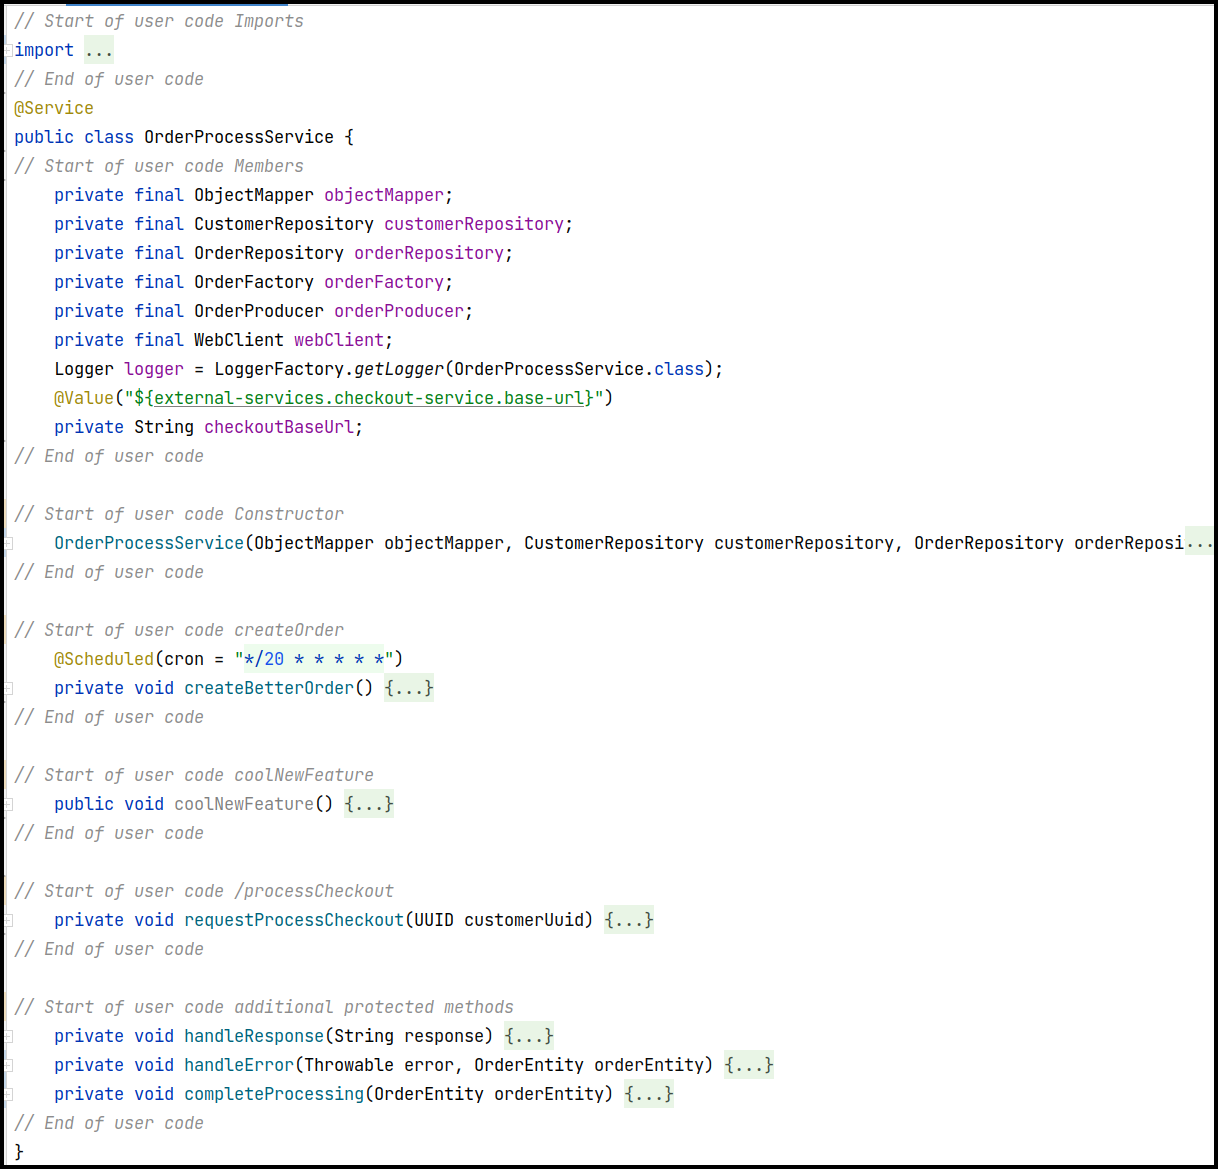
\includegraphics[width=\textwidth]{bilder/gen/1_light.png}
\caption{Generierter Code mit geschützten Bereichen}
\end{figure}

\newpage

Hierbei ist hervorzuheben, dass die Methode \glqq coolNewFeature()\grqq{} erst nach der initialen Codegenerierung dem Modell als Verhalten hinzugefügt wurde. Dabei blieb bestehender Code erhalten. Der durch das Verhalten neu generierte wurde problemlos hinzugefügt.
Das Löschen dieses Verhaltens aus dem Modell führt ebenfalls zu einer funktionierenden Entfernung der Methode und deren Implementierung. Das Umbenennen würde hingegen zum Verlust der Implementierung führen.

Alternativ zu diesem feingranulareren Ansatz ist es auch möglich, ganze Klassen als einen einzigen geschützten Bereich zu kennzeichnen. Exemplarisch wurde dies in einem dem Quellcode anhängenden Beispielprojekt \cite{bspprojekt}, welches einen Microservice enthält, für Entity und Repository umgesetzt. In diesem ist ebenso die in Abbildung 6.1 abgebildete Service-Klasse zu finden.

\subsection{Open Rewrite}

Eine weitere Möglichkeit, solche Migrationen durchzuführen, ist die Verwendung der Software OpenRewrite \cite{rewrite}. Sie kann über eine Gradle- oder Maven-Build-Konfiguration in ein Projekt eingebunden werden und ermöglicht es, bereits existierende Migrationsrezepte zu nutzen. Diese erlauben einfache Refactorings, wie das Umbenennen eines Pakets, einer Methode oder das automatische Formatieren von Code. Auch komplexere Rezepte, die eine Codebasis vollständig auf eine aktuelle Java-Version migrieren können, existieren. Zudem können eigene Rezepte in Java implementiert werden. Ergänzend zur Implementierung mit AQL-geschützten Bereichen sollen nun exemplarisch einige Rezepte vorgestellt werden. Diese wurden ebenfalls dem Beispielprojekt hinzugefügt.

\begin{lstlisting}[caption=OpenRewrite Rezepte]
---
type: specs.openrewrite.org/v1beta/recipe
name: app.ChangeMethod
displayName: Change method name example
recipeList:
  - org.openrewrite.java.ChangeMethodName:
      methodPattern: app..* createOrder()
      newMethodName: createBetterOrder
      
---
type: specs.openrewrite.org/v1beta/recipe
name: app.order
recipeList:
  - org.openrewrite.java.ChangePackage:
      oldPackageName: app.order
      newPackageName: app.ordernew
\end{lstlisting}

In der rewrite.yml werden neue Namen für das Ändern von Methodennamen und das Umstrukturieren von Paketen innerhalb der Rezepte definiert.

\newpage

\begin{lstlisting}[caption=Anwenden von OpenRewrite Rezepten]
rewrite {
    activeRecipe(
            'app.order',
            'app.ChangeMethod',
            'org.openrewrite.java.format.AutoFormat'
    )
}
\end{lstlisting}

In der build.gradle können diese dann mit dem vorher definierten Rezeptnamen referenziert werden. Auch Rezepte wie das automatische Formatieren von Code, die keine weitere Konfiguration verlangen, können hier genutzt werden. Durch das Anwenden des Gradle-Tasks \glqq rewriteRun\grqq{} werden diese nun ausgeführt.

Somit können auch speziellere Migrationen, die sich nicht durch Änderungen des Modells umsetzen lassen, durchgeführt werden.